\chapter{State of the Art}

This chapter describes how the company handles the required processes and takes advantages of the technologies in order to develop the software that runs on the industrial devices and the cloud platform. It also describes the standards and regulations that the company must comply with.

\section{Company}

The company where we did our internship is located in the province of Verona in Italy. The factory building formally includes the main company, which is the one that designs and produces the industrial devices, and another company.

The latter is the business where we are enrolled for the internship; it is in charge of the development of cloud platform that allows these devices to become domotic, that is industrial automation, in order to send and receive data from the cloud, to be able to interact with the device remotely and to be able to monitor the status of the device. The software is a built-in service running on the hardware, and all the data are collected and sent to the cloud through the company's servers.

Since the businesses are under the same holding group, they share administrative resources and also technical resources. From now on, we refer to the main (or first) company talking about standards, regulations and devices, and to the (our) second one talking about the software and the cloud.

\subsection{Software company organization}

The cloud management software, developed by the second company, is composed of five main layers and it is managed by five different teams:
\begin{itemize}
  \item \textbf{Device data}: it should make friendly the adoption of the platform and it handles the cloud lifecycle of a device, by managing the device registration and the handling of the collected data to being able to create flexible dashboards and reports;
  \item \textbf{VPN}: it handles the connection to a device through a VPN and it is in charge of the security of the connection;
  \item \textbf{Apps}: the work of the apps team is to increase the value of the platform, by allowing third parties to integrate their services with the platform and by creating apps that can be installed on the devices. Customers can craft their own apps by using the provided \textit{Software Development Kit} (SDK), that is a set of tools and documentation;
  \item \textbf{Core}: it is the core of the platform and it in responsible for the provided backend REST APIs mainly used for the frontend website. It also handles the management of the user via a custom \textit{IDentity Provider} (IDP);
  \item \textbf{Platform}: last but not least, the platform team orchestrate all the infrastructure needed to run the services and it is in charge of the deployment of the services on the cloud. It is also responsible for the monitoring of the services and for the security of the development lifecycle and deploy process.
\end{itemize}

The cloud software is developed using the microservices architecture, that is a design pattern that structures an application as a collection of loosely coupled services. Services can be developed, deployed and scaled independently.

We were virtually part of the apps team, and we were in charge of developing a scanning tool that can be used to check the security of the devices powered by the cloud management software and to report the potential issues to the customer.

\section{Initial design}

Under the hood, every PLC is powered by a custom Linux distribution, provided by \textit{Yocto Project}, an open-source collaboration project that helps developers create custom Linux-based systems regardless of the hardware architecture~\cite{yocto-project}, developed by the internal \textit{Research \& Development} (R\&D) team.

In order to be able to make the device interact with the industrial machines, the company provides a proprietary IDE software, needed to scratch projects and deploy them on the device. This software lets the user define the inputs and outputs of the device and the logic that will be executed on the device. In example, the user can define a trigger, an alarm that will be raised when a certain condition is met, a personalized handling of the data received by the many supported protocols and so on.

Furthermore, the same IDE is used to draw the graphical interface that will be displayed on the HMI and to define the behaviour of the interface itself.\\
The graphical interface is composed of widgets, that are the building blocks of the interface. The user can define the position of the widgets, their size, their colour and their behaviour. The widgets can be buttons, labels, images, graphs or custom-defined ones.

The setup with their IDE software is strictly related to the device interacting with the industrial machines, and it is not the focus of the internship project. The focus is on the device itself, and on the software that runs on it.

Given that, at the beginning stages, our scanning tool could not be installed and released as a firmware update for the devices, because that would require a modification of the R\&D team's workflow, we decided to develop the scanning tool as an executable binary that can be run on the device itself. It is a \textit{command-line interface} (CLI) tool able to perform the scan and report an output to the user. Then, the user will be able to fix the issues by itself, by interacting with the device settings.

\section{Device settings}

The PLC backend provides a web interface that can be used to view and change the system settings of the device. The user can change the network settings, set the datetime, set the management user password, manage the startup of the services like the SSH server and much more. The HMI touchscreen, through dedicated gestures, lets the user directly interact locally with the onboard interface, otherwise it is possible to reach it by connecting to the device's network address. \\
Client and server, respectively the graphical interface and the backend, are independent of each other; the web interface is powered by REST APIs.

For the internship project, we will take advantage of the REST APIs to retrieve the status of the device and to potentially change its settings. Internally to the company, the APIs are documented with the \textit{OpenAPI Specification}, formerly \textit{Swagger Specification}, that is an API description format that depicts the endpoints, the parameters, the responses, the authentication needed to call them and licenses or other information. The Swagger file can be visualized through the Swagger UI, a web interface that renders OpenAPI definitions as interactive documentation.~\cite{openapi-swagger}

% We can devise two different scenarios: API calls made by a remote host over a network and API calls made by the local host. In the first case, the TLS protocol secures the communication using the public-key authentication first, and then the APIs are protected by a basic authentication, that is the client must provide a management username and its related password. In the second case, the web server listens over a port only accessible by the same host with no further authentication needed.
% TODO: Note about use-cases and security of this approach

\section{Standards and Regulations}
Until the so-called third industrial age, or Industry 3.0, cybersecurity had minimal impact on manufacturing. Industrial machinery wasn't necessarily connected to the internet or each other, making external risks unlikely. However, with the dawn of Industry 4.0, smart machinery and smart factories have become vital for the smooth operation of production departments, placing cybersecurity at the forefront of concern.

Cybersecurity involves protecting systems, networks and programs from digital attacks. Given the critical nature of the topic and the attention it demands, companies are embarking on paths to elevate their awareness of cyberattacks, adopting internal policies, or even pursuing specific certifications in cybersecurity. Concurrently, national and international legislators have introduced new legislative measures imposing new obligations on certain entities concerning cybersecurity.

Let's now consider the most recent legislative measures on cybersecurity and the related certifications that manufacturing industries must take into account.\\
Certifications provide a guarantee of product and company security. The main certifications currently considered include:
\begin{itemize}
  \item \textbf{IEC 62443}: This series of international standards is renowned for enhancing the security of industrial control systems, setting forth fundamental prerequisites to shield industrial systems from cyber threats;
  \item \textbf{ISO/IEC 27001 (2022)}: This certification covers various aspects, including security policy, human resource security, physical and environmental security, communications management and regulatory compliance;
\end{itemize}

There are then several laws and regulations that address under various profiles the issue of cybersecurity among them it is worth noting:~\cite{cybersecurity-standards-regulations-compliance}
\begin{itemize}
  \item \textbf{Cyber Resilience Act (CRA)}~\footnote{\url{https://eur-lex.europa.eu/legal-content/EN/TXT/?uri=celex:52022PC0454}}: While still pending final approval by the European Institutions, the Cyber Resilience Act seeks to enhance the resilience of the European digital market by ensuring that connected devices and digital services are equipped to withstand cyberattacks effectively. It will become effective in 2027;
  \item  \textbf{NIS Directive 2}~\footnote{\url{https://eur-lex.europa.eu/legal-content/EN/TXT/?uri=CELEX:32022L2555}}: This directive outlines essential criteria that companies must adhere to in order to maintain a robust level of cybersecurity. These criteria cover the implementation of risk analysis strategies, fortification of information system security and effective incident management protocols. EU Member States must transpose this directive, with enforcement specified in the respective national acts;
  \item \textbf{Italian Cybersecurity Law (June 28th, 2024 No. 90)}~\footnote{\url{https://www.gazzettaufficiale.it/eli/id/2024/07/02/24G00108/sg}}: This Italian law pertains to national cybersecurity and applies to both public and private entities whose services are deemed critical. It mandates the implementation of security measures to protect critical digital infrastructures and sensitive information, including specific obligations to notify the Cybersecurity Agency of any cyber incidents;
  \item \textbf{New Machinery Regulation No. 1230/2023}~\footnote{\url{https://eur-lex.europa.eu/legal-content/EN/TXT/?uri=CELEX:32023R1230}}: This regulation will replace the Machinery Directive No. 2006/42/EC, focusing on the overall safety of machinery and semi-machinery and it will become effective in 2027. It emphasizes the essential integration of cybersecurity into the design and manufacturing processes of machinery, recognizing the potential risks that cyber vulnerabilities pose to physical safety;
\end{itemize}

This chapter will provide an overview of the most relevant standards and regulations for the context of the internship's research, focusing on the industrial sector and the required goals; in particular, we will detail more about \textit{IEC 62443}, \textit{ISO 27001}, \textit{NIS 2} and \textit{CRA}.

\subsection{IEC 62443}
\label{sec:iec-62443}

The IEC 62443 provides guidelines, rules and definitions specifically crafted for any Industrial Automation and Control Systems (IACS). Compared to ISO 27001, it is more focused on the specific sector instead of being more universal and open for interpretation depending on the company it applies to.

The market requires the IEC 62443 certification for the companies that are involved in the production of industrial devices, as it is a guarantee of the security of the product and the company itself.

The IEC 62443 is a set of standards drafted by the \textit{Internation Electrotechnical Commission} (IEC) and it is divided into four categories:~\cite{understanding-iec-62443-parts}
\begin{enumerate}
  \item \textbf{General}: it covers topics that are common to the entire series;
  \item \textbf{Policies and procedures}: focuses on methods and processes associated with IACS security;
  \item \textbf{System}: it covers the requirements for the secure development and integration of systems;
  \item \textbf{Component}: it covers the requirements for the secure development and integration of components.
\end{enumerate}

\begin{figure}[t]
  \centering
  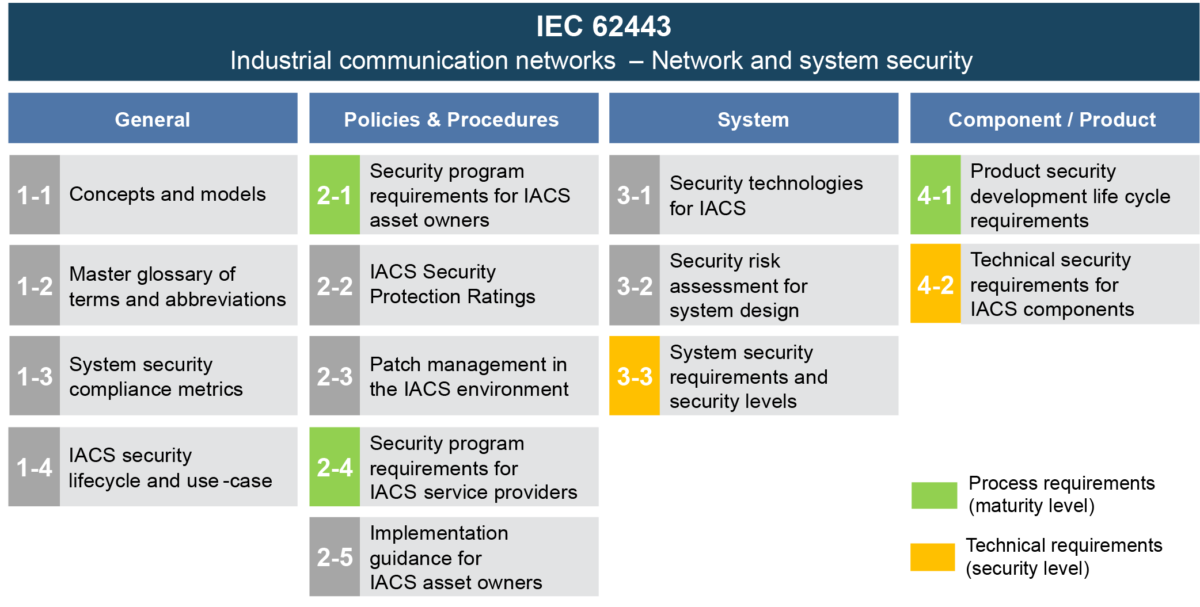
\includegraphics[width=0.9\textwidth]{chapters/03/assets/iec62443.png}
  \caption[IEC 62443 Parts and Sections. Image by Mohamed Wassef O. \protect\footnotemark]{IEC 62443 Parts and Sections. Image by Mohamed Wassef O. \protect\footnotemark}
  \label{fig:iec-62443}
\end{figure}
\footnotetext{\url{https://www.linkedin.com/pulse/power-iec-62443-safeguarding-industrial-automation-othmani-gsrde}}

Each category is divided into several subcategories, corresponding to different subjects and requirements. The IEC 62443 is a comprehensive standard that covers all the specific aspects starting from the product design up to the development.

Each subcategory, identified by the category number followed by an increasing index, contains a list of System Requirements (SR) that the company must meet to obtain the certification.

In example, a system requirement taken from the subcategory \textit{System security requirements and security levels} (\texttt{3-3}) is the one shown in~\cref{fig:iec62443_3-3_3_9}. We are going to explain it in detail.

The SR 3.9 states the following:
\begin{mdframed}
  SR 3.9 - Protection of audit information: The control system shall protect audit information and audit tools (if present) from unauthorized access, modification and deletion.
\end{mdframed}\label{sr:3-3_3-9}

Log audits are essential for the prevention and detection of cyberattacks. When something goes wrong, the log audit can help to understand what happened, when and where it happened and who was involved. This is a fundamental requirement for the IEC 62443 certification.

For each Security Requirement listed in the documentation, the standard also describes some potential rationale and supplemental guidance to help the company understand the requirement and how to implement it.

Each SR is made of four security levels. \\
A Security Level (SL) is a measure of the security of a system or component, which is eventually transmitted to the final client. It is a score from 1 to 4, where 1 indicates the lowest complexity of the solution we can apply to follow the requirement, and 4 indicates the highest complexity.~\cite{ixon-practical-guide-iec-62443}

It is possible to increase the score of the security level by applying more non-trivial solutions, expressed as a \textit{Requirement Enhancement}. An enhancement to increase the security level from 3 to 4 is stated in \texttt{SR 3.9 RE 1}:
\begin{mdframed}
  SR 3.9 RE 1 - Audit records on write-once media: The control system shall provide the capability to produce audit records on hardware-enforced write-once media.
\end{mdframed}\label{sr:3-3_3-9_re1}

We would like to note that not every SR has exactly four RE; instead, it could be that there are less solutions in order to increase its score. For instance, this is the case for the SR 3.9, which has only one RE and the minimum applicable security level is the level 2, as shown in~\cref{fig:iec62443_3-3_3_9}.

\begin{figure}[t]
  \centering
  \fbox{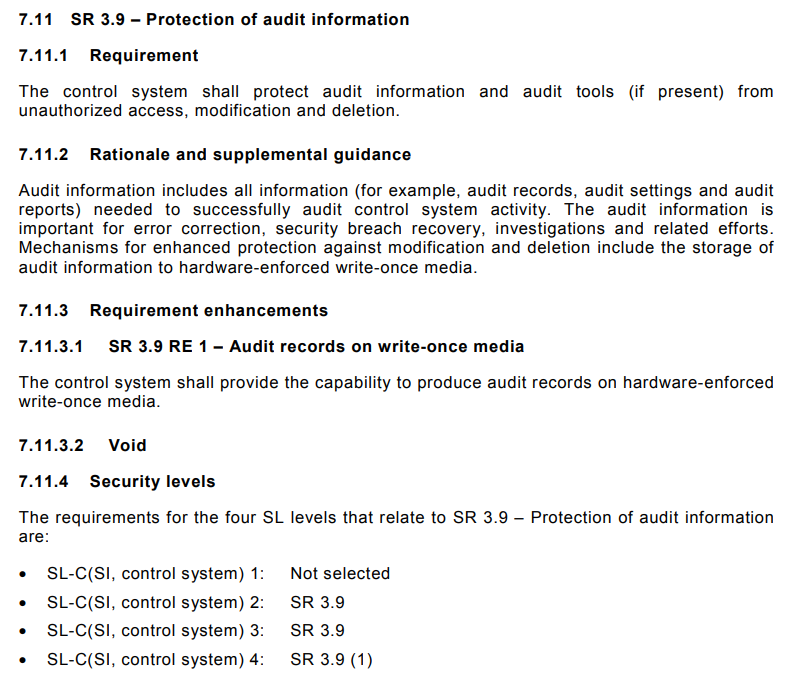
\includegraphics[width=1.0\textwidth]{chapters/03/assets/iec62443_3-3_3_9.png}}
  \caption[Snapshot of a System Requirement]{Snapshot of a System Requirement}
  \label{fig:iec62443_3-3_3_9}
\end{figure}

Moreover, sometimes the highest security level is not always the best solution or the most suitable for the company. Therefore, it is essential to evaluate the cost and the benefits of the solution before applying it.


In the context of the company we are working with and the internship project we are involved in, because we are directly at the level of product design and component development and deployment, the relevant subcategories we are focusing on are \texttt{3-3}, \texttt{4-1} and \texttt{4-2}, respectively named \textit{System security requirements and security levels}, \textit{Product security development life cycle requirements} and \textit{Technical security requirements for IACS components}.

At the system level, \texttt{IEC 62443-3-3} introduces security levels and corresponding requirements, offering a scalable framework to protect industrial systems. This part enables organizations to customize their security measures based on specific risk profiles and operational demands.

\texttt{IEC 62443-4-1} lays the foundation for secure product development, emphasizing the critical importance of incorporating security measures right from the design phase. It encourages manufacturers to adopt a security-centric approach to product development, ensuring that components are fortified against cyber threats from the very beginning.

Moving from development to deployment, \texttt{IEC 62443-4-2} specifies the technical security requirements for IACS components. It defines essential security capabilities such as robust authentication, encryption and intrusion detection, ensuring that each component reinforces the overall security of the system.~\cite{iec-62443-safeguarding-industrial-automation-linkedin}


\subsection{ISO/IEC 27001}

The ISO/IEC 27001 is a globally recognized standard addressed to companies of any size and from all sectors of activity with guidance for establishing, implementing, maintaining and continually improving an information security management system, which is a set of policies and procedures defining and managing controls that an organization needs to implement to ensure that it is sensibly protecting the confidentiality, availability and integrity of assets from threats and vulnerabilities. An information security management system that meets the requirements of ISO/IEC 27001 preserves the CIA triad and gives confidence to interested parties that risks are adequately managed.

Conformity with this standard means that an organization or business has put in place a system to manage risks related to the security of data owned or handled by the company and that this system respects all the best practices and principles enshrined in this International Standard.

It has been jointly published by the \textit{International Organization for Standardization} (ISO)~\cite{iso} and the \textit{International Electrotechnical Commission} (IEC)~\cite{iec}. The number indicates that it was published under the responsibility of Subcommittee 27 (on Information Security, Cybersecurity and Privacy Protection) of ISO's and IEC's Joint Technical Committee on Information Technology (ISO/IEC JTC 1).

It is widely used around the world; as per the ISO Survey 2022, over 70000 certificates were reported in 150 countries and from all economic sectors, ranging from agriculture through manufacturing to social services.~\cite{iso-27001}

\subsection{NIS Directive 2}
\label{sec:nis-directive-2}

The Network and Information Security (NIS) Directive is the first piece of EU-wide legislation on cybersecurity, drawn in 2016, and its specific aim was to achieve a high common level of cybersecurity across the Member States. To respond to the growing threats posed by digitalisation and the surge in cyber-attacks, the Commission has submitted a proposal to replace the NIS Directive and thereby strengthen the security requirements, address the security of supply chains, streamline reporting obligations and introduce more stringent supervisory measures and stricter enforcement requirements, including harmonised sanctions across the EU. NIS 2 entered into force on January 2023, and the Member States have until October 2024 to transpose its measures into national law.

The major key features of the updated directive are:~\cite{nis2-directive-faqs}
\begin{itemize}
  \item \textbf{Expanded scope}: NIS2 extends its scope to cover more sectors and industries. It applies to essential and important entities: the former include energy (electricity, district heating and cooling, oil and gas), transport (air, rail, water and road), banking, health, pharmaceutical, water, digital infrastructure (internet exchange points, DNS providers, TLD name registries, cloud computing service providers, data centre service providers, content delivery networks), public administration and space. The latter include postal and courier services, waste management, chemicals, food, manufacturing of medical devices, computers and electronics, machinery equipment, motor vehicles and digital providers (online marketplaces, online search engines and social networking service platforms).\\
        Anyway, Essential and Important entities are deemed to be under the jurisdiction of the Member State where they provide their services
  \item \textbf{Incident Reporting}: Companies must report significant cybersecurity incidents within 24 hours of detection, improving coordination between national cybersecurity authorities and helping mitigate the impact of attacks.
  \item \textbf{Fines and Penalties}: NIS2 introduces higher penalties for non-compliance, similar to the GDPR, with fines that could reach up to 2\% of an organization's total global turnover.
\end{itemize}

NIS 2 aims to enhance the resilience of the European digital market, ensuring the continuity of essential services even in the face of sophisticated cyberattacks.

\subsection{Cyber Resilience Act}

While the cybersecurity of providers of digital services is regulated at EU level by the NIS Directive 2, as analyzed in~\cref{sec:nis-directive-2}, the security of products with digital elements and software products is so far not subject to any comprehensive piece of EU regulation.~\cite{cra-eu}

Therefore, the European Commission proposed the Cyber Resilience Act in 2022; it has been approved in early 2024~\cite{cra-timelinel} and manufacturers have to place compliant products on the Union market by 2027, aiming to enhance the security of ICT products, services and processes.

It applies to products connected directly or indirectly to another device or network except for specified exclusions such as open-source software or services that are already covered by existing rules, which is the case for medical devices, aviation and cars. A non-exhaustive list of products that are in scope of the CRA includes:~\cite{cra-overview}
\begin{itemize}
  \item \textbf{end devices}: laptops, smartphones, cameras, smart equipments, network equipments, Industrial Automation Control Systems (IACS);
  \item \textbf{software}: firmware, operating systems, applications;
  \item \textbf{components}: components like CPUs, video cards and libraries;
\end{itemize}

% With all being said, we now move to the next chapter, where we discuss how the directives and the standards we have just analyzed are applied in the context of the company we are working with and the internship project we are involved in.

\section{\textit{Go} programming language}

\textit{Go} is an open-source programming language supported by Google, designed for building simple, reliable and efficient software. It is statically typed, compiled and syntactically similar to C, with the added benefits of built-in concurrency management, garbage collection, memory safety and a robust standard library plus packages. Go is widely used in cloud computing and web development due to its simplicity, performance and scalability.~\cite{go-lang-site}~\cite{go-lang-wikipedia}\\
Go was released in 2007 by Google, and at the time of writing it is at version \texttt{1.22}.

% \begin{figure}[h]
%   \centering
%   
\includegraphics[width=0.9\textwidth]{chapters/03/assets/golang}
%   \caption{Go logo and mascot. Taken from \texttt{nixsolutions.com}}
%   \label{fig:go-logo-mascot}
% \end{figure}

Go's standard library provides comprehensive support for networking, encryption and concurrency. The built-in packages for HTTP, TLS and JSON processing simplify the implementation of RESTful APIs, secure communication channels and data serialization/deserialization, respectively. If additional functionalities are required, the language supports third-party packages through the Go module system; in order to download a custom package, the developer simply references it in the code via the link to the repository and the Go compiler will automatically download and install it.

Go also offers a robust testing framework to write unit tests and benchmarks to ensure the reliability and performance of their code. The testing framework is integrated into the language and provides a simple and efficient way to write tests for functions and methods. The testing framework also supports the generation of code coverage reports to identify untested code paths and improve the overall test coverage. Furthermore, Go's testing framework supports the use of table-driven tests, which allow the developer to define test cases in a structured format and iterate over them to execute the tests and also it supports fuzzing, a technique used to discover vulnerabilities in software by providing random or invalid inputs to the program.

Another point in favor is the efficiency of the language. Go is compiled into machine code, which makes it faster than interpreted languages like Python. The language's garbage collection mechanism automatically manages memory allocation and deallocation, reducing the risk of memory leaks and improving the overall performance of the application. The language is more than a full order of magnitude faster than Python, with a smaller memory footprint and faster execution times.~\cite{go-lang-performance}

One of the main reasons for choosing Go for the internship project is its versatility in building executable binaries for multiple platforms, including Windows, macOS and Linux. Go's cross-compilation capabilities allow the developers to build binaries for different operating systems and architectures from a single codebase, simplifying the deployment process and ensuring compatibility across various platforms. Given that industrial devices run on different architectures and operating systems, the ability to build cross-platform binaries is essential. The language natively supports the binaries compilation for over 50 combinations of operating systems and architectures~\cite{go-lang-compilation-combo}; given that the majority of the company's devices run either on \texttt{Arm 32bit} or \texttt{Arm 64bit} or \texttt{x86 64bit} architectures, the Go compiler can generate the executables for these architectures with no further configuration needed.

